\documentclass[12pt,a4paper]{book}
\usepackage[latin1]{inputenc}
\usepackage{amsmath}
\usepackage{amsfonts}
\usepackage{amssymb}
\usepackage{makeidx}
\usepackage{pdfpages}
%\usepackage{fullpage}
\usepackage[left=1cm,right=2cm,top=2cm,footskip=1.5cm,bottom=1cm]{geometry}
\usepackage{listings}
\usepackage{color}

%\setlength{\parskip}{\baselineskip}  
\setlength{\parindent}{0pt} 

\definecolor{lightgray}{gray}{0.97}
\lstset{frame=single}
\lstset{framesep=5pt}
\lstset{language=C++}
\lstset{keywordstyle=\color{black}\bfseries\emph}
\lstset{backgroundcolor=\color{lightgray}}

\author{Uwe Rathmann}
\title{Qwt Plot Framework}


\begin{document}

\maketitle
\pagestyle{headings}

\tableofcontents

\chapter{Introduction}

Introduction bla bla

\chapter{Plot Widget}

\section{Composite Widget Architecture}

QwtPlot is a composite widget, that contains a QwtPlotCanvas, 
4 QwtScaleWidgets, a QwtTextWidget for the title and an optional QwtLegend. 
All widgets might be hidden or visible depending on the current configuration 
of the plot widget. Many attributes of a plot are in fact 
attributes of the internal child widgets,
\\
\\
QwtPlot has its own layout engine, that is implemented as QwtPlotLayout. 
The following picture shows a layout of a plot widget, where all internal widgets are visible.

\bigskip
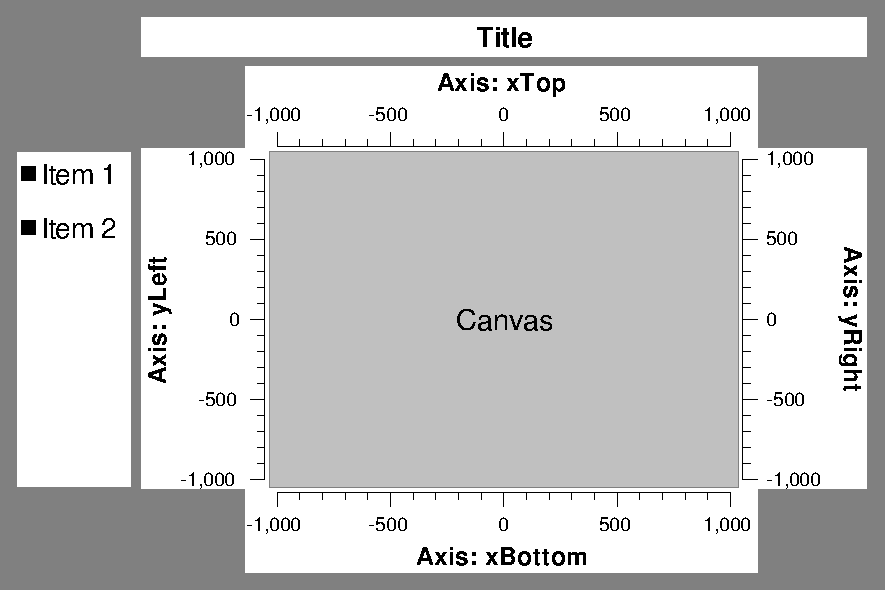
\includegraphics[scale=1.0]{plotlayout.pdf}
\bigskip

The composite widget architecture\footnote{Subject of redesign} 
of QwtPlot has some consequences for the programming interface:

\begin{itemize}

\item Attributes\\
Most attributes of child widgets or the layout object can't be 
changed using QwtPlot methods. Instead the application code has to 
use a getter method for the child and access it directly. 
Beside making the programming interface less obvious it has the effect, 
that the plot can't be configured in the designer ( or creator )

\footnote{A proof of concept has been made how to embed a special 
editor for QwtPlot into the designer and how to pass the edited 
properties using QwtPlot::applyProperties() - but it was never implemented.}.

\item Events\\
Overloading event callbacks of QwtPlot has no effect when an event is posted to a child widget. When the application wants to implement a specific event handling it needs to use a technique called event filtering.

\end{itemize}

\begin{lstlisting}
#include <qwt_plot.h>
#include <qwt_plot_canvas.h>
#include <qwt_scale_widget.h>

class MyPlot: public QwtPlot
{
public:
    MyPlot(QWidget *parent = NULL);
    
    virtual bool eventFilter(QObject *obj, QEvent *event)
};

MyPlot::MyPlot(QWidget *parent):
   QwtPlot(parent)
{
    for ( int axis = 0; axis < QwtPlot::axisCnt; axis++ )
    	axisWidget(axis)->setFont( QFont( ... ) );

	canvas()->setPalette( QPalette( Qt::darkBlue ) );
    canvas()->installEventFilter(this);
} 

bool MyPlot::eventFilter(QObject *object, QEvent *event)
{
    if ( object == canvas() )
    {
        ...
    }
    return QwtPlot::eventFilter(object, event);
}
\end{lstlisting}


\section{Scale Widget}
\section{Legend}



\chapter{Scales, Axes and Transformations}

\section{Scale Divisions}

\section{Scale Maps}

\section{Scale Engine}

\section{Scale Renderer}

\chapter{Navigation and Selection}

\section{Picking}
\section{Zooming}
\section{Panning}

\chapter{Items on the Plot Canvas}

Decorations + items representing some sort of data.

\section{Overview}
\section{The Grid}
\section{Axes}

\section{Markers for Coordinates or Points}
\section{Curves displaying a series of 2D Points}

\subsection{Symbols}
\subsection{Styles}
\subsection{Curve Fitting}


\section{Curves displaying a series of 3D Points}
\section{Curves displaying a series of intervals}
\section{Histograms displaying ...}

\section{Spectrograms and other items displaying raster data}

\section{SVG Item}

\chapter{Exporting and Printing}

\chapter{Text Engines}

All Qwt widgets use QwtText objects to specify text labels. 
Their format attribute specifies the text engine, that is 
responsible for interpreting and rendering the string. 
Today there are 3 different text engines available.
\footnote{A text engine for TeX documents would be a great 
solution to display labels in mathematical notation. 
There are a couple Qt/KDE applications available, 
that can display TeX documents. Most of them simply write 
the TeX document to a file generate an image from it using the 
TeX tools and load the image then - but maybe there is 
somewhere an "real" implementation inside, that 
translates a TeX document to QPainter calls. }

\begin{itemize}

\item Plain Text\\
QwtPlainTextEngine doesn't take care of any syntax and lays out and renders 
the string using QPainter and QFontMetrics.

\item Rich Text\\
QwtRichTextEngine is able to display a subset of HTML 4 markup using the renderer,
that is built into the Scribe classes of Qt. It is often used because of
sub- or superscripts to display very simple mathematical expressions.

\item Mathematical Markup Language (MathML)\\
QwtMathMLTextEngine uses the MathML renderer from the Qt solutions
\footnote{
Unfortunately we don't know much about the quality of the MathML renderer yet
as it is not much in use because of earlier license issues. 
Today the solution package is LGPL'd like the rest of Qt and in Qwt 6 it can be
installed and used easily.
}
package. In MathML it should be able to define almost any kind of formula

\end{itemize}

The text engines for plain and rich texts are always available. 
The MathML text engine ( like any other homebrew text engine ) has to be
registered by the application code:

\bigskip 
\begin{lstlisting}
#include <qwt_mathml_text_engine.h>

QwtText::setTextEngine(QwtText::MathMLText, new QwtMathMLTextEngine());
\end{lstlisting}
\bigskip 

QwtText might also have a couple of additional properties, controlling how to display a text.

\begin{itemize}
\item Font
\item Color
\item Background color and border pen
\end{itemize}


\chapter{Advanced Topics}

\section{Incremental Painting}

\section{Building Plot Grids}

\section{Controlling the Aspect Ratio}

\section{Levels of Detail}

\end{document}
